\documentclass[%
12pt, %
final, % 
oneside, % 
onecolumn, %  
centertags]{article} % относится к классу article и размер шрифта 12 пунктовб, {article: статья, report: отчеты и диссертации, book: книга, letter: письмо}

% \usepackage{fontspec}
 
% \setmainfont{Times New Roman}

% \documentclass[a4paper, 12pt]{report}

\topmargin= -30pt % насколько сверху будет страница
\textheight= 650pt


\usepackage[utf8]{inputenc} % задает кодировку, utf-8 кодировка, включающая в себя знаки почти всех языков мира
\usepackage[english]{babel} % подключает необходимые языки, основным языком является английский

\selectlanguage{english} % настройки будут на английском, но писать будет на русском

\usepackage{euscript}
\usepackage{supertabular}

\renewcommand{\baselinestretch}{1.0} 

\usepackage[colorlinks=true,linkcolor=blue,unicode=true,urlcolor = blue]{hyperref} %hypered
\usepackage[pdftex]{graphicx} % для графики

\usepackage{amsthm, amssymb, amsmath, amsfonts} % математический пакет, математические шрифты
\usepackage{textcomp}
\usepackage[noend]{algorithmic}
\usepackage[ruled]{algorithm}
\usepackage{lipsum}
\usepackage{indentfirst}
\usepackage{babel}
\usepackage{pgfplots}
\usepackage{setspace}
\usepackage{xcolor}
\usepackage{hyperref}
\usepackage{subfigure}

\setcounter{secnumdepth}{5}
\setcounter{tocdepth}{5}
\newcommand\simpleparagraph[1]{%
  \stepcounter{paragraph}\paragraph*{\theparagraph\quad{}#1}}
\usepackage{listings}
% \usepackage{xcolor}
%\usepackage{minted}

\lstset { %
     language=C++,
     backgroundcolor=\color{black!5}, % set backgroundcolor
     basicstyle=\footnotesize,% basic font setting
}


\linespread{1.0} 
\setlength{\parindent}{2.4em}
\setlength{\parskip}{0.1em}

\pgfplotsset{compat=1.9}
\pgfplotsset{model/.style = {blue, samples = 100}} 
\pgfplotsset{experiment/.style = {red}}

\theoremstyle{plain}
\binoppenalty=10000

\newtheorem{theorem}{Theorem}[section] % theorem

\theoremstyle{definition}
% \newtheorem{definition}{Определение}[subsection]
\newtheorem{definition}{Definition}[subsection]

\theoremstyle{remark}
% \newtheorem{remark}{Замечание}[section]

% \newtheorem{corollary}{Следствие}

% \newtheorem{proposition}{Proposition}

% \newtheorem{example}{Пример}

% \newtheorem{lemma}{Лемма}[section]

\renewcommand*{\proofname}{Proof}

\graphicspath{ {./images/} }


% \usepackage{amsmath,amsfonts,amssymb, setspace}  % Разнообразные математические команды и значки
% \usepackage{indentfirst}     % Отступ в первом абзаце

% \pagestyle{empty}
\usepackage[left=2.5cm, right=1.5cm, top=2.5cm, bottom=2.5cm]{geometry}
\usepackage[medium]{titlesec}
\usepackage{graphicx}
% \graphicspath{ {./images/} }

\begin{document}

	\begin{titlepage} 
		\begin{center}
		\textbf{}\\[2.0cm]
		\LARGE FEDERAL STATE AUTONOMOUS EDUCATIONAL INSTITUTION OF HIGHER EDUCATION \\[0.5cm]
		\Large ITMO UNIVERSITY \\[3cm]
		\LARGE Report\\
		\Large MPI. Assignments $6-7$ \\
		\Large Parallel algorithms for the analysis and synthesis of data \\[4cm]


		\begin{flushright}
		Performed by\\
		Aleksandr Shirokov\\
		J4133c\\
		Accepted by\\
		Petr Andriushchenko

		Deadline: 20.12.21
		\end{flushright}

		\vfill 

		{\Large {St. Petersburg}} \par
		{\Large {2021}}
		\end{center} 
	\end{titlepage}

\tableofcontents
\newpage


\section{Assignments}

\subsection{Assignment 6. MPI. Retrieving information about the message attributes.}

\subsubsection{Formulation of the problem}

\begin{enumerate}
	\item Compile the example \textsc{Assignment6.c} in detail, run it and explain it.
	\item Transform the program using the \textsc{MPI\_TAG} field of the status structure in the 
condition.
\end{enumerate}

\subsubsection{Example of launch parameters and output. Detailed description of solution}

Code for \textbf{assignment 6} is \href{https:\//github.com/aptmess/parallel_algorithms/blob/master/HT/hw_mpi/Assignment6.c}{here}.

Compilation example: \textsc{mpic++ -o ./cpf/6.o Assignment6.c}

Launch example: \textsc{mpirun --oversubscribe -np 4 ./cpf/6.o}

\begin{center}
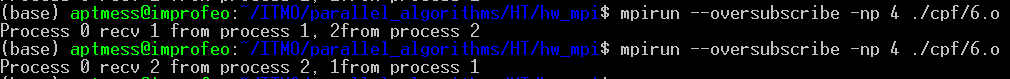
\includegraphics[scale=0.7]{6.1.png}

There could be only two results of program output
\end{center}

Let's move to the the code and explain how it works.

\begin{center}
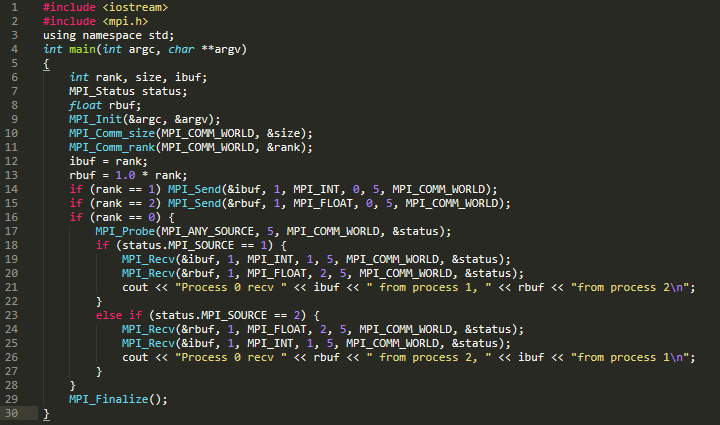
\includegraphics[scale=0.9]{6.code.png}

Assignment6 code
\end{center}

Firstly there is an initialization of parallel part using \textsc{MPI\_Init}, after if rank of process is $1$ then the int $1$ will be send as a message and if rank of process is $2$, then the float value $2.0$ will be send as message. After we are going to main process $0$ logic: 

\begin{itemize}
	\item \textsc{MPI\_Probe} this function is waiting for message from any process with $\operatorname{msgtag}=5$ and wouldn't go next if the message doesn't come to process $0$. Let's make it clear - function only understand that message come to process, but doesn't get it.
	\item After that if \textsc{status.MPI\_SOURCE == 1} so if first was message from process $1$ then there is a print message that $1$st process's message was quicklier, else - that the second was quicklier and the value from second process will be displayed first.
\end{itemize}

After I have transformed the problem using \textsc{MPI\_TAG} field. Here are results:

\begin{center}
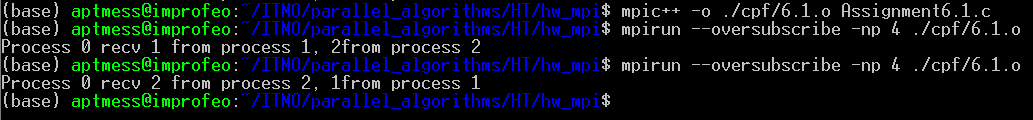
\includegraphics[scale=0.65]{6.2.png}

Results are the same. Take a look at code
\end{center}

Code for \textbf{assignment 6.1} is \href{https:\//github.com/aptmess/parallel_algorithms/blob/master/HT/hw_mpi/Assignment6.1.c}{here}.

Compilation example: \textsc{mpic++ -o ./cpf/6.1.o Assignment6.1.c}

Launch example: \textsc{mpirun --oversubscribe -np 4 ./cpf/6.1.o}

\begin{center}
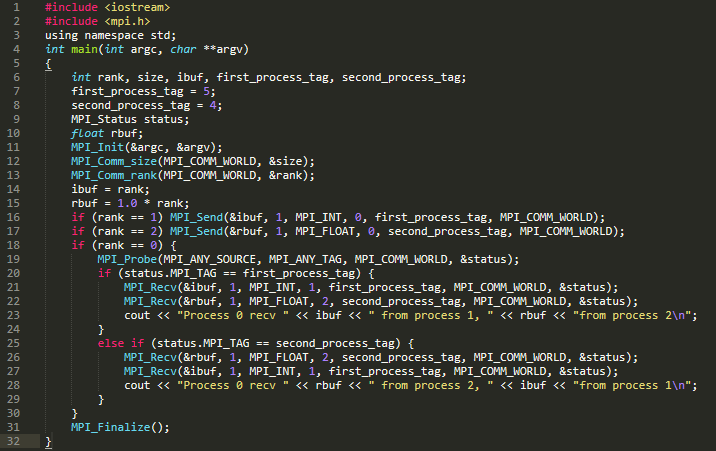
\includegraphics[scale=0.7]{6.2.code.png}

Assignment6 part II code
\end{center}

Everything is more or less the same, but now we are expecting any tag in \textsc{MPI\_Probe} function and processes $1$ and $2$ has different tags ($5$ and $4$) and condition is also have changed (\textsc{status.MPI\_TAG}). Program works correctly.


\newpage
\subsection{Assignment 7. MPI. Dot product of vectors.} 

\subsubsection{Formulation of the problem}

\begin{enumerate}
	\item Write an MPI program that implements the dot product of two vectors distributed between processes.
	\item Two vectors with a size of at least 1,000,000 elements are initialized at process $0$ and filled with “1”, then they are sent in equal parts to all processes. 
	\item Parts of vectors are scalar multiplied on each process, the result is sent to the root process and summed up.
	\item The total is displayed.
\end{enumerate}

Scalar product for two vectors $a = [a_1, \ldots, a_n]$ and $b = [b_1, \ldots, b_n]$ in $n$-dimensional space defined as:

$$a \cdot b = \sum\limits_{i=1}^n a_i b_i = a_1b_1 + \ldots + a_nb_n$$


\begin{figure}[h]
\begin{center}
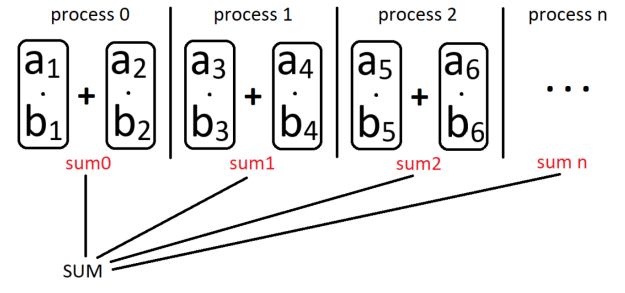
\includegraphics[scale=1]{7_how_to_solve.png}

The algorithm of parallel dot product

\label{labl}
\end{center}
\end{figure}


\subsubsection{Example of launch parameters and output. Detailed description of solution}

Code for \textbf{assignment 7} is \href{https:\//github.com/aptmess/parallel_algorithms/blob/master/HT/hw_mpi/Assignment7.c}{here}.

Compilation example: \textsc{mpic++ -o ./cpf/7.o Assignment7.c}

Launch example: \textsc{mpirun --oversubscribe -np 4 ./cpf/7.o 1000000}

\begin{center}
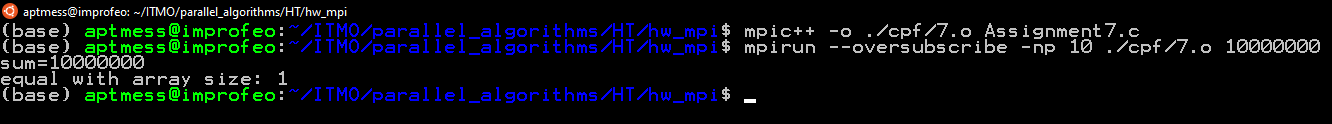
\includegraphics[scale=0.5]{7.1.png}
\end{center}

\begin{center}
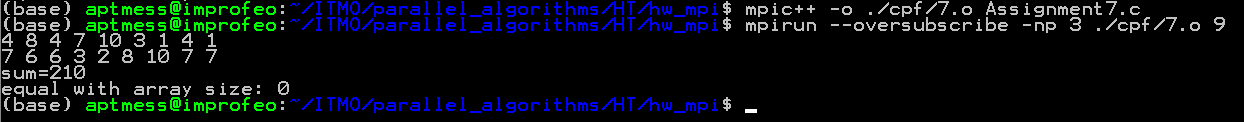
\includegraphics[scale=0.55]{7_t.png}

Some testing of function not on only ones
\end{center}

Let's move to the the code and explain how it works.

\begin{figure}[h!]
\centering
\subfigure{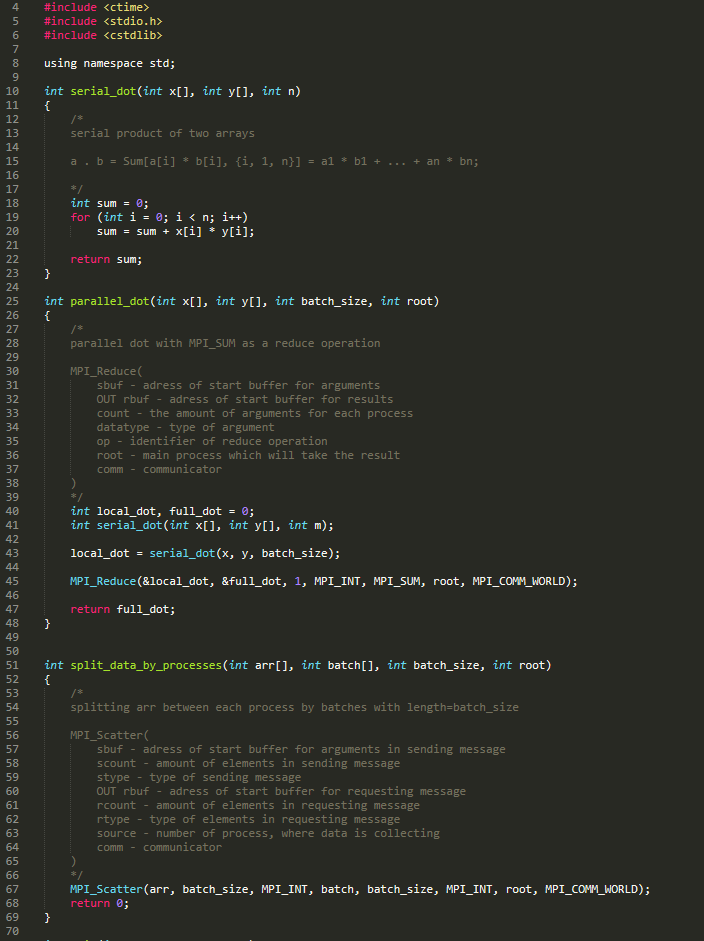
\includegraphics[width=0.42\textwidth]{7.2.png}} 
\subfigure{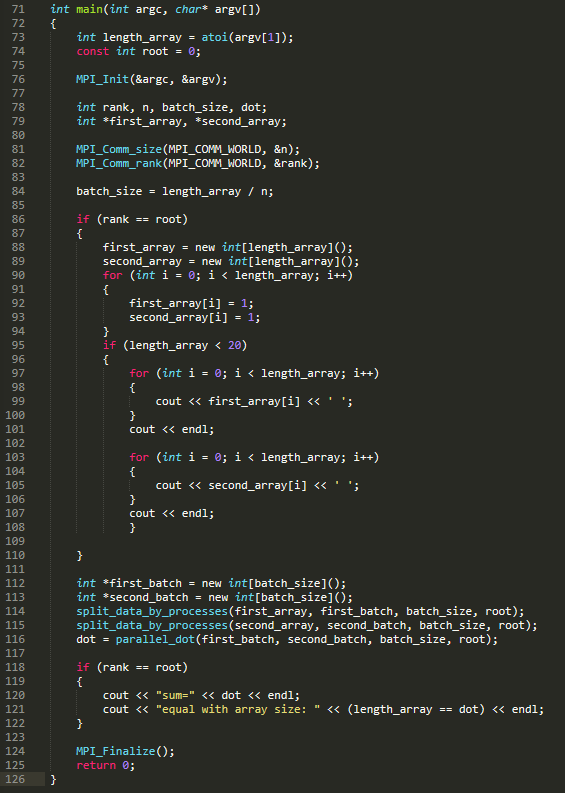
\includegraphics[width=0.4\textwidth]{7.3.png}} 


Assignment7 code
\end{figure}

On picture in section \nameref{labl} there are a structure of algorithm - we should split our arrays into different processes, map some function inside processes such as \textsc{serial\_dot} and collect (reduce) result in the main process $0$ - this algorithm our program is doing. On the left picture there are three functions:

\begin{itemize}
	\item \textsc{serial\_dot} which calculate the dot product of two vectors;
	\item \textsc{parallel\_dot} which run \textsc{serial\_dot} function and after that with \textsc{MPI\_Reduce} function reduce results from local variable to \textsc{sbuf} variable - \textsc{full\_dot}.
	\item \textsc{split\_data\_by\_processes} which splitts the input array between each process by \textit{batches} with the length of \textit{batch\_size}
\end{itemize}

Have to mentioned that for correct work of algorithm the amount of processes should be a divider of length of array. Batch size is $\frac{\operatorname{length\_of\_array}}{\operatorname{amount\_of\_processes}}$.

The main function is using this functions - firstly in root process $0$ we initialize the arrya of length \textsc{length\_array} and fill them $1$, after that we initializing batch, split data for each process by batch size for every process, in each process serial dot is running and sending to main process, which collect the dot variable - sum of each serial dot in processes. Then root process show result and check that sum is equal to size of array (because each array is filled by $1$). Program works correctly.


\subsection{Appendix}

The link to the sourse code which is placed on my \href{https://github.com/aptmess/parallel_algorithms}{github}.


\end{document}